\documentclass{article}
\usepackage{graphicx}
\usepackage{listings}
\usepackage{xcolor}
\usepackage{hyperref}
\usepackage{geometry}
\geometry{a4paper, margin=1in}

\title{Grafici dell'utilizzo di memoria heap da parte degli algoritmi di ricerca}
\author{Adriano Oliviero}
\date{\today}

\begin{document}

\maketitle

\tableofcontents

\section{Grafici e Risultati}
Di seguito sono riportati alcuni grafici che visualizzano i risultati sperimentali degli algoritmi di ricerca applicati ai dataset:

\subsection{com-lj.ungraph}
\subsubsection{breadth-first}
\begin{figure}[h]
	\centering
	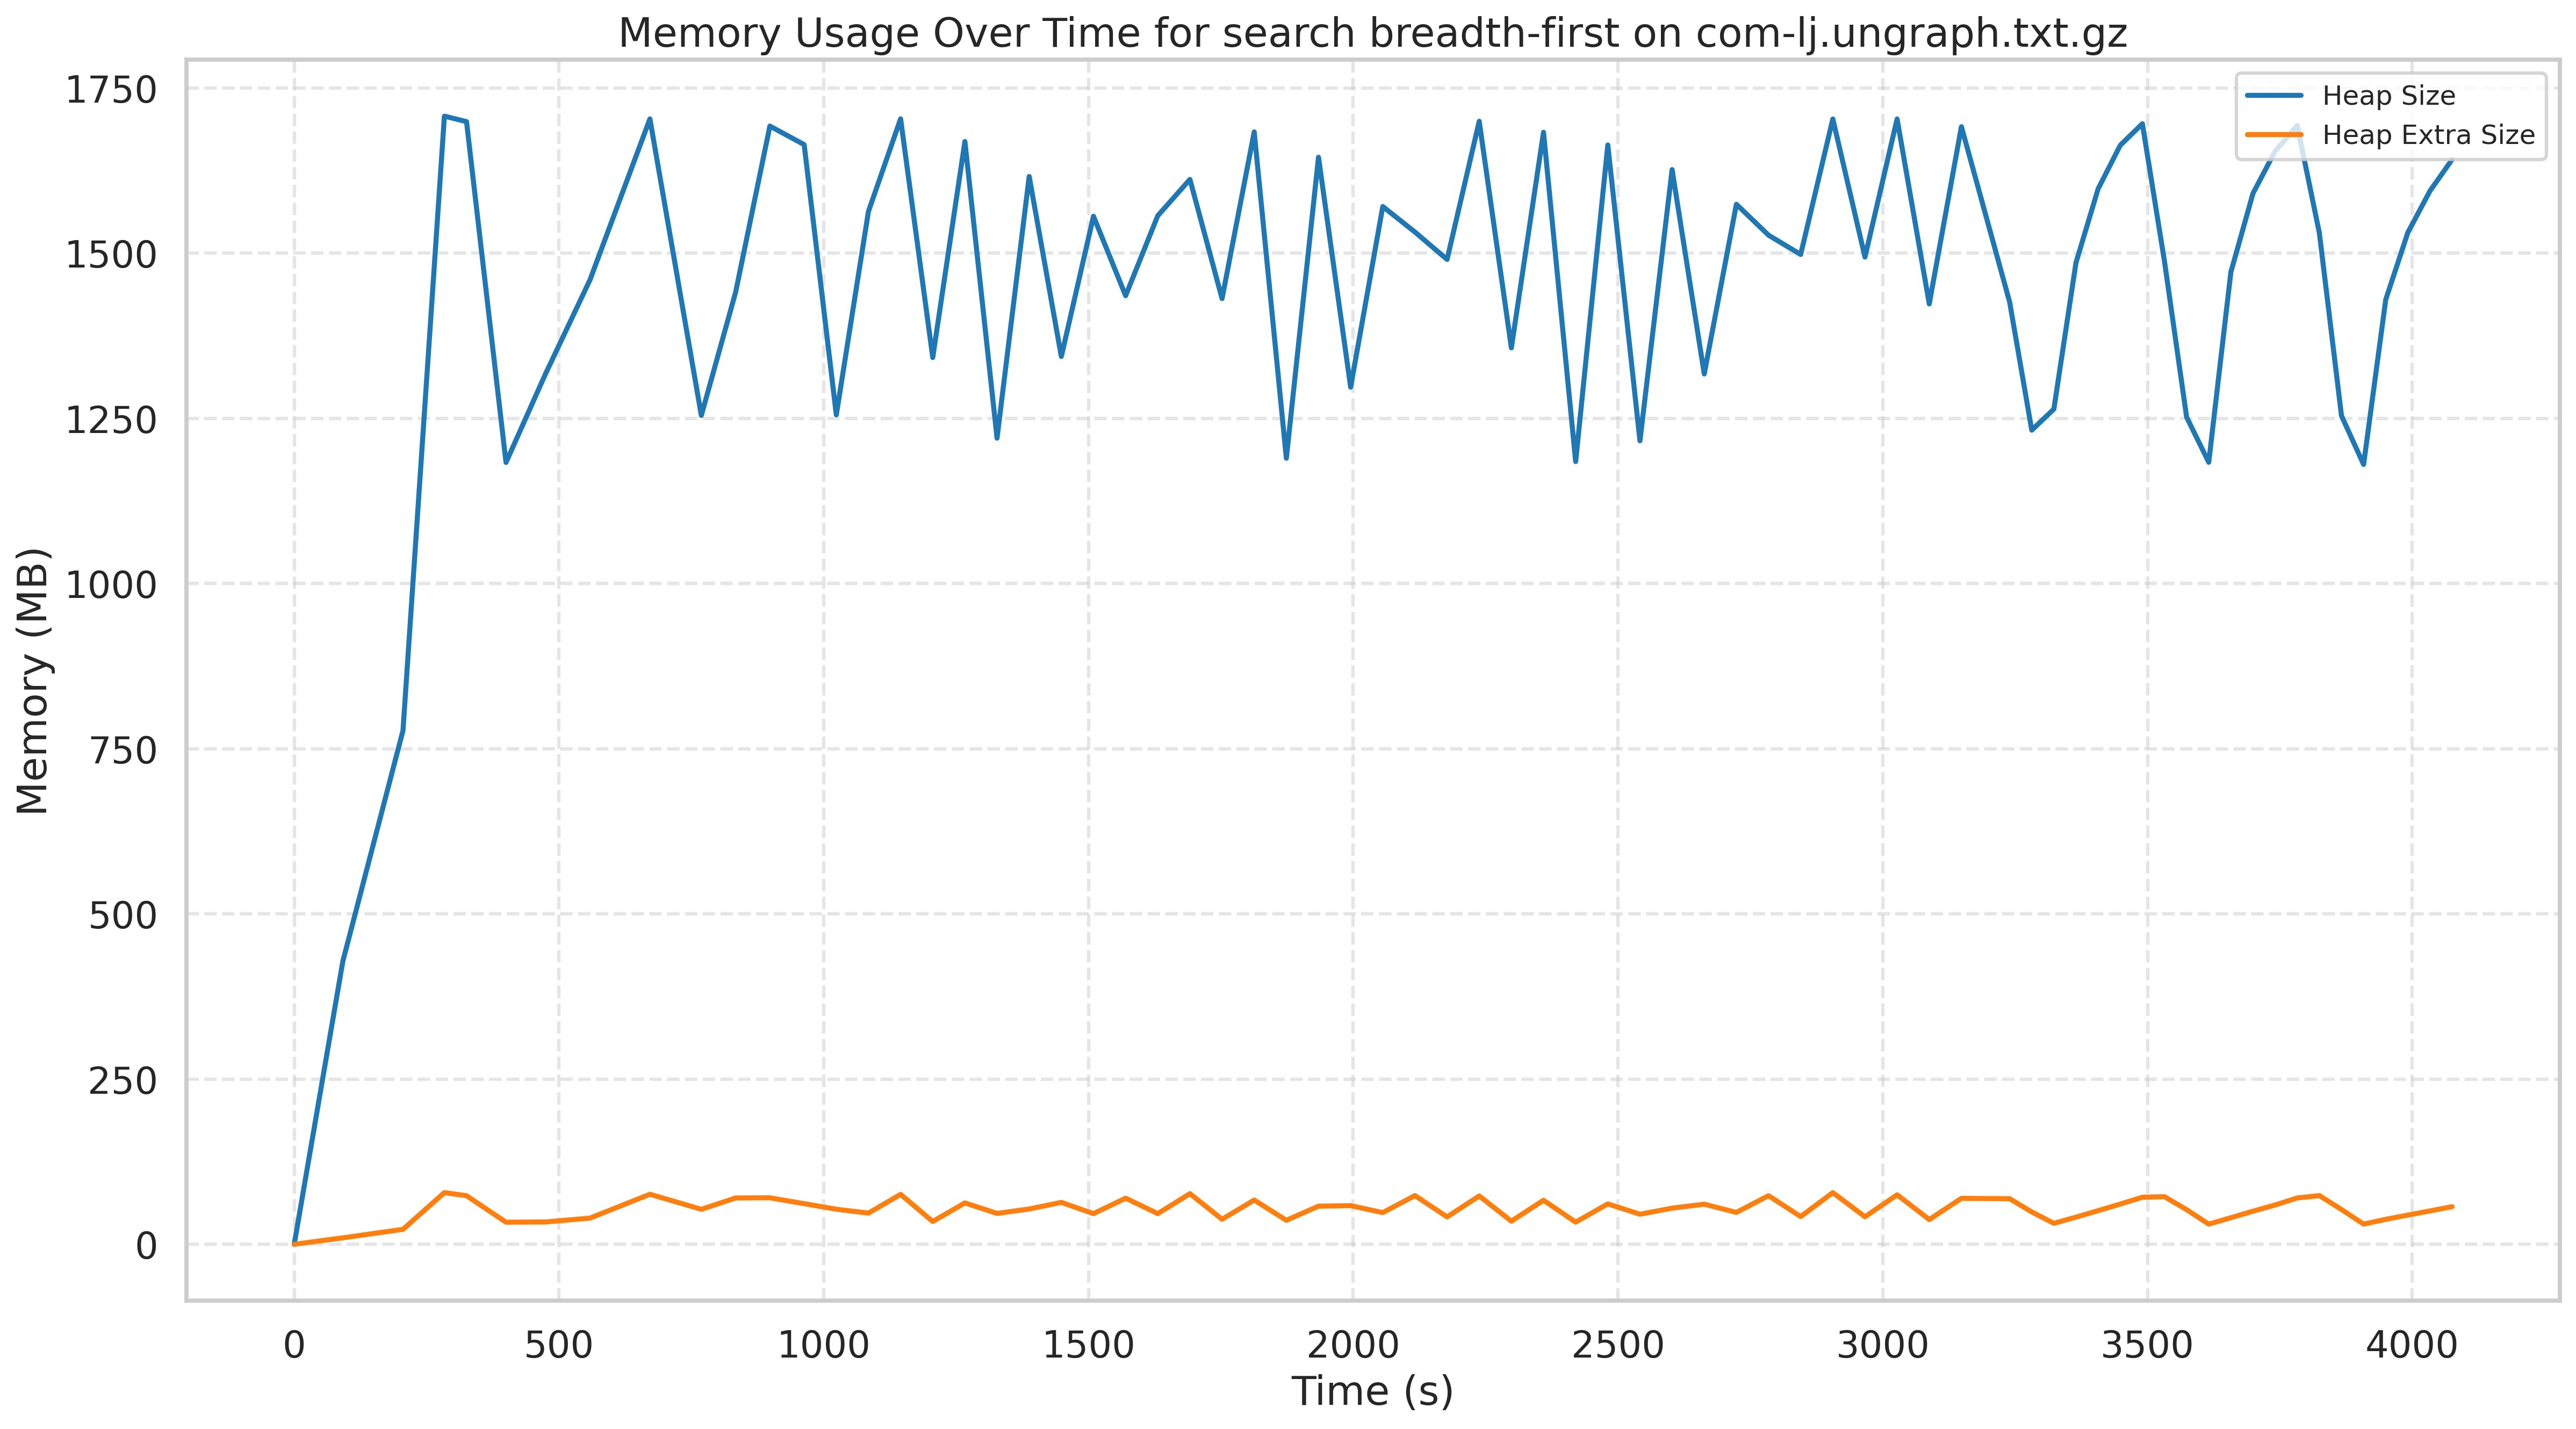
\includegraphics[width=\textwidth]{../plots/com-lj.ungraph_breadth-first.png}
	\caption{Grafico: breadth-first su com-lj.ungraph}
\end{figure}
\end{document}

